\section{按 KV 块分组}

相邻 query 分组是先固定一组 query，再看它们的选块是否重叠。也可以反过来：每个 CTA 负责一个 KV 块， 处理所有选中这个块的 query。 例如图 2(c) 中的 A 被 $q_0$ 和 $q_2$ 选中，它们不相邻，仍然能共享同一份 K/V。 外层遍历 KV 块、内层遍历 query，一般叫做 KV-outer 循环顺序。

MSA 采用 KV-outer 的方法计算 Sparse Attention。KV-outer 下每块 K/V 只读一次，代价变成每个 query 要为每个选中的块 读一次 Q、写一份局部输出，最后再读回合并。按第 3 节同样的口径， 每个 query 的访存约为 $6Gkd$ 字节，而有效计算仍是 $4GdkB_k$ FLOPs，两者之比约为 $\tfrac{2}{3}B_k$。 只要 $\tfrac{2}{3}B_k \gg G$，KV-outer 的算术强度就远高于 Q-outer 的 $G$。

具体实现上，先把“每个 query 选了哪些块”转换成“每个块被哪些 query 选中”的反向索引： 统计每个块被选中的次数，用前缀和确定写入位置，再填入 query 编号。 主 kernel 按这个索引分批读入 Q，K/V 一直留在 shared memory 中重复使用（图 7）。 单个 query 只贡献 $G$ 行，所以要把同一块的多个 query 拼进一个 MMA 填满 $M$ 维。 KV-outer 下这样拼没有代价，因为它们用的是同一份 K/V\hyperlink{ref-9}{\textsuperscript{[9]}}。

\begin{figure}[!htbp]
\centering
\resizebox{\linewidth}{!}{%
\begin{tikzpicture}[x=1cm,y=1cm,font=\small,
 flow/.style={-{Stealth[length=1.6mm]},draw=accent,line width=.7pt}]
\node[anchor=west,font=\bfseries] at (0,6.55) {按 KV 块分组：负责 block A 的一个 CTA};
\node[font=\footnotesize,text=muted] at (1.5,5.98) {HBM：原始张量};
\node[font=\footnotesize,text=muted] at (4.9,5.98) {SMEM：输入 tile};
\node[font=\footnotesize,text=muted] at (9.2,5.98) {TMEM：MMA 的中间结果};
\draw[dashed,ink] (3.4,1.25) rectangle (12.15,5.68);
\foreach \x/\name in {.35/K_A,1.83/V_A}{
 \foreach \r in {0,1,2}{\foreach \c in {0,1,2}{
  \draw[fill=selected,draw=white] (\x+\c*.32,4.41+\r*.28) rectangle ++(.32,.28);
 }}
 \node[font=\footnotesize] at (\x+.48,5.48) {$\name$};
}
\draw[flow] (1.4,5.34) -- (4.29,5.34);
\draw[flow] (2.88,4.5) -- (5.92,4.5);
\foreach \x/\name in {4.35/K_A,6.0/V_A}{
 \foreach \r in {0,1,2}{\foreach \c in {0,1,2}{
  \draw[fill=selected,draw=white] (\x+\c*.3,4.66+\r*.28) rectangle ++(.3,.28);
 }}
 \node[font=\footnotesize] at (\x+.45,4.25) {$\name$};
}
\foreach \i in {0,1,2}{
 \draw[fill=waste,draw=white] (.45,3.17-\i*.53) rectangle ++(1.52,.44);
 \node[font=\footnotesize] at (1.21,3.39-\i*.53) {$Q_{\i,g}$};
}
\foreach \i in {0,2}{
 \draw[fill=selected,draw=accent] (.45,3.17-\i*.53) rectangle ++(1.52,.44);
 \node[font=\footnotesize] at (1.21,3.39-\i*.53) {$Q_{\i,g}$};
}
\foreach \r/\q in {0/2,1/0}{
 \draw[fill=selected,draw=accent] (4.15,2.23+\r*.47) rectangle ++(1.7,.43);
 \node[font=\footnotesize] at (5,2.445+\r*.47) {$Q_{\q,g}$};
}
\draw[flow] (2.03,3.39) -- (4.07,2.915);
\draw[flow] (2.03,2.33) -- (4.07,2.445);
\node[font=\scriptsize] at (2.88,1.92) {按表搬入 Q};
\node[font=\footnotesize] at (5,3.55) {$Q_{\mathrm{batch}}:(M G)\times d$};
\draw[flow] (5.93,2.65) -- (7.52,2.65) -- (7.52,4.7);
\draw[flow] (5.32,5.05) -- (5.66,5.05) -- (5.66,5.57) -- (7.52,5.57) -- (7.52,5.05) -- (7.64,5.05);
\node[font=\scriptsize,fill=white] at (7.45,4.45) {QK / MMA};
\foreach \r in {0,1,2}{\foreach \c in {0,1,2}{
 \draw[fill=selected,draw=white] (7.72+\c*.35,4.61+\r*.28) rectangle ++(.35,.28);
 \draw[fill=statefill,draw=white] (10.27+\c*.35,4.61+\r*.28) rectangle ++(.35,.28);
 \draw[fill=statefill,draw=white] (10.27+\c*.35,2.58+\r*.28) rectangle ++(.35,.28);
}}
\node[font=\footnotesize] at (8.24,5.62) {$S$};
\node[font=\footnotesize] at (10.80,5.62) {$P$};
\draw[flow] (8.95,5.05) -- (10.13,5.05);
\node[font=\scriptsize,align=center] at (9.55,4.3) {寄存器中\\mask / softmax};
\draw[flow] (10.80,4.52) -- (10.80,3.56) node[midway,right,font=\scriptsize] {PV / MMA};
\draw[flow] (6.45,4.0) -- (6.45,3.0) -- (10.1,3.0);
\node[font=\footnotesize] at (10.8,2.21) {$O_{i,A}$ 与 $L_{i,A}$};
\draw[flow] (11.47,3.0) -- (12.63,3.0) node[midway,above,font=\scriptsize] {写回};
\foreach \r/\q in {0/2,1/0}{
 \draw[fill=statefill,draw=stateedge] (12.73,2.5+\r*.51) rectangle ++(1.55,.46);
 \node[font=\scriptsize] at (13.5,2.73+\r*.51) {$O_{\q,A},L_{\q,A}$};
}
\node[font=\footnotesize,align=center] at (13.5,4.17) {HBM\\局部结果};
\node[font=\footnotesize,text=muted] at (7.75,1.68) {K/V 留在片上，一批批换 Q};
\draw[flow] (13.5,2.33) -- (13.5,.75) -- (10.63,.75);
\node[font=\footnotesize] at (8.5,.75) {合并局部结果};
\draw[flow] (6.36,.75) -- (5.58,.75);
\draw[fill=selected,draw=accent] (4.32,.51) rectangle ++(1.1,.48);
\node[font=\footnotesize] at (4.87,.75) {$O_i$};
\node[anchor=west,font=\footnotesize,text=muted] at (.1,-.02) {建反向表 $\rightarrow$ 各 CTA 算局部结果 $\rightarrow$ 合并};
\end{tikzpicture}
}
\setcounter{figure}{6}
\caption{按 KV 块分组时一个 CTA 的数据流：K/V 留在片上，按反向索引分批读入 Q，局部结果写出后再合并。}
\label{fig:kv-kernel}
\end{figure}
\FloatBarrier

好处是不再有被 mask 的计算。问题在于一个 query 的结果分散在多个 CTA 中， 每个 CTA 只算了它的一部分 softmax，不能直接相加。 FSA 和 MSA 都把计算和合并拆成两个 kernel，以避免跨 CTA 的 atomic 累加\hyperlink{ref-11}{\textsuperscript{[11]}}\hyperlink{ref-9}{\textsuperscript{[9]}}， 但处理 softmax 的方式不同。FSA 先用一个单独的 kernel 预先算好每个 query 的 softmax 统计量； MSA 则让每个 CTA 写出局部输出和 log-sum-exp（LSE），由 combine kernel 按 LSE 加权合并， 做法和 FlashDecoding 的 split-KV 相同。我们采用后一种。 所以额外开销有四项：构建反向索引、不连续地读取 Q、写出并读回局部结果，以及最后的合并。

还有一个 Q-outer 没有的问题：负载不均衡。有些块几乎被所有 query 选中，比如序列开头的 sink 块， 一个 CTA 处理它要花的时间远超其他块。MSA 用一个调度 kernel 把热门块沿 query 维切成多段， 分给多个 CTA，并预先为每段分配好局部结果的写入位置\hyperlink{ref-9}{\textsuperscript{[9]}}。

\subsection{实测}

按 KV 块分组同样依赖重叠程度。选中同一块的 query 越多，K/V 的复用越充分； 选块越分散，每个 CTA 分到的 query 越少，需要读取的不同块也越多。 我们在 B200 上测量了这一点：4K 个 query 的 prefill，prefix 长度从 1K 增加到 1M， 每个 query 的选块数固定，只改变 query 之间的重叠程度。三档重叠下，有效计算量完全相同。

\begin{figure}[!htbp]
\centering
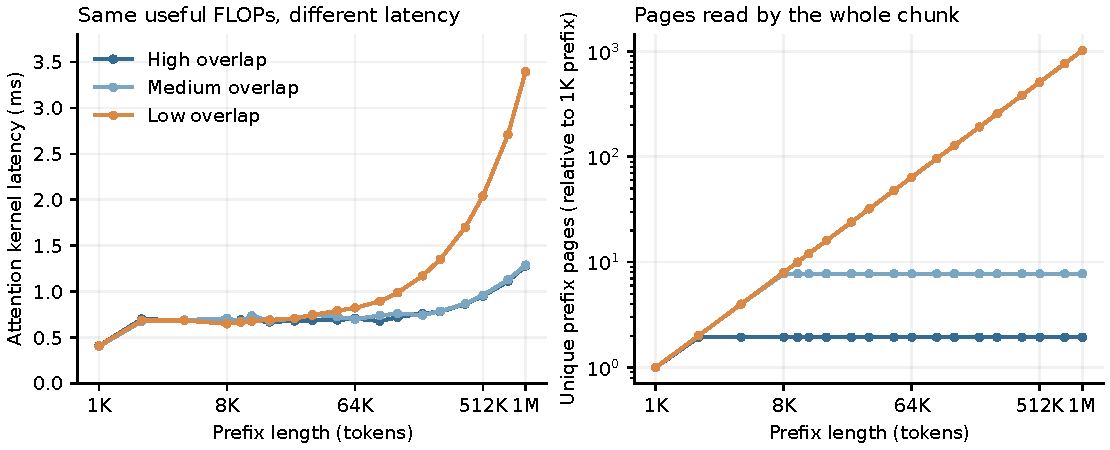
\includegraphics[width=\linewidth]{figures/kv-owner-overlap.pdf}
\setcounter{figure}{7}
\caption{B200 上的重叠度扫描。左：attention kernel 耗时；右：全部 query 读取的不同 KV 块数，以 1K prefix 为 1。}
\label{fig:kv-owner-overlap}
\end{figure}
\FloatBarrier

图 8 中，prefix 不超过 32K 时三条线几乎重合，因为可选的块本来就不多。 之后低重叠的耗时明显上升。到 1M prefix，高重叠的 attention 耗时 1.28 ms， 低重叠几乎读遍了所有块，耗时 3.40 ms，是前者的 \textbf{2.66 倍}， 算力利用率（相对 BF16 稠密峰值）从 9.4\% 降到 3.5\%。 构建反向索引只多花 0.14 ms，合并步骤的耗时不变，差距几乎都在主 kernel 中。

中等重叠这一档最能说明问题：它的平均重叠度只有 0.26，看起来很分散， 但读取的不同块数始终只有高重叠的 4 倍，耗时也和高重叠几乎相同。 \textbf{预测耗时，读取的不同块数比平均重叠度更准。} cache 命中可能是原因：FSA 也指出，KV-outer 下不连续地读取 Q 会拉低 L2 命中率\hyperlink{ref-11}{\textsuperscript{[11]}}:

\begin{quote}\small
for one KV block, only a subset of total query tokens is involved for attention computation, and query token indices are typically non-contiguous.

non-contiguous memory access leads to a lower L2 cache hit rate, thereby reducing effective memory bandwidth and degrading overall kernel efficiency.
\end{quote}
